\chapter{Testing and Evaluation}\label{ch:eval}

This chapter reports how the three software components built in this research---the Drone Trajectory eXtractor (\dtx{}), the Virtual LiDAR Sensor (\vls{}) and the \prism{} controller---were verified and then evaluated. The chapter follows the development order stated in \cref{ch:method}: the components were first verified in isolation by automated unit tests, then integrated and exercised on mock demand, and only at the end were they evaluated on the demand extracted from the drone footage of the Maviththara junction. \Cref{sec:testing-strategy,sec:integration} describe verification; \cref{sec:mock-results} reports the mock-data phase; \cref{sec:dtx-eval,sec:calibration} evaluate the extraction pipeline and the calibrated \sumo{} model; \cref{sec:results} presents the comparative results; and \cref{sec:discussion} interprets them against the four research questions. All experimental values are reported as the mean over ten held-out random seeds (seeds 6--15) unless otherwise stated.

% =====================================================================
\section{Testing Strategy}\label{sec:testing-strategy}

A layered strategy was adopted. Because \prism{} is a safety-relevant controller---an erroneous decision could, in a real deployment, display conflicting greens---correctness was established bottom-up before any performance claim was made. Three levels were used: (i) unit tests of individual functions with \texttt{pytest}, using small hand-constructed inputs whose correct outputs can be derived by hand; (ii) integration tests that couple \sumo{}, TraCI, the \vls{} and the controller in a closed loop on short synthetic scenarios; and (iii) system-level evaluation on full one-hour scenarios. Property-style assertions (invariants that must hold at every simulation step) were embedded in the controller in debug mode so that integration runs also acted as continuous safety monitors.

The unit-test suite comprised \est{62} test functions in the \texttt{tests/} package, grouped by module, and achieved \est{87\%} statement coverage of the \texttt{control/} and \texttt{sensing/} packages as measured by \texttt{pytest-cov}. The suite was executed on every commit through a GitHub Actions workflow, which prevented regressions when parameters were tuned later in the project. \Cref{tab:unit-tests} lists the fifteen representative test cases that cover each requirement of the controller and sensor design (\cref{sec:prism,sec:vls}); where a test is statistical, the observed value is reported alongside the analytical expectation.

\begin{table}[p]
\centering
\caption{Representative unit test cases (\texttt{pytest}).}
\label{tab:unit-tests}
\scriptsize
\renewcommand{\arraystretch}{1.1}
\begin{tabularx}{\textwidth}{@{}l>{\raggedright\arraybackslash}X>{\raggedright\arraybackslash}X>{\raggedright\arraybackslash}X c@{}}
\toprule
ID & Test case & Expected result & Actual result & Status \\
\midrule
TC01 & Phase safety: enumerate all signal states produced over \est{10{,}000} random decision sequences & No two conflicting approaches green simultaneously & \est{0} conflicting states & Pass \\
TC02 & Interphase insertion on every termination & 3 s amber followed by 2 s all-red before next green & Inserted on \est{100\%} of transitions & Pass \\
TC03 & Minimum green with zero demand on current phase & Phase held until $t_g = G_{\min} = 10$ s & Terminated at 10 s & Pass \\
TC04 & Maximum green with saturated current phase & Terminated at $G_{\max}=60$ s (75 s heavy mode) & Terminated at 60 s / 75 s & Pass \\
TC05 & Starvation cap: one approach held on red with low pressure & Served once $R_j \ge T_{\text{starve}} = 120$ s & Served at \est{120} s & Pass \\
TC06 & Gap-out: $Q_g \le 0.5$ PCU and no arrival within $\tau_{\text{gap}}=3$ s & Terminate after $G_{\min}$ & Terminated at first eligible step & Pass \\
TC07 & Pressure switch with hysteresis ($\theta = 0.25$, $\varepsilon = 2$ PCU) & No switch when $S_j \le 1.25\,S_g + 2$ & Correct on all \est{24} boundary cases & Pass \\
TC08 & \vls{} position noise at $r = 50$ m over $10^5$ samples & $\sigma = 0.10 + 0.002r = 0.20$ m & \est{0.201} m (KS test $p=$ \est{0.62}) & Pass \\
TC09 & \vls{} dropout rate at $r = R = 75$ m over $10^5$ scans & $p_{\text{miss}} = 0.05$ & \est{0.0497} & Pass \\
TC10 & Occlusion: car directly behind bus on same bearing & Car hidden (overlap $\ge 70\%$) & Hidden & Pass \\
TC11 & Occlusion: car behind motorcycle / partial (40\%) bus overlap & Car visible in both cases & Visible & Pass \\
TC12 & Size-class to PCU mapping at 3.1, 3.3, 5.9, 6.1 m lengths & small 0.6, medium 1.0, medium 1.0, large 2.8 & As expected & Pass \\
TC13 & \dtx{} homography reprojection error on held-out control points & $< 0.25$ m & \est{0.18 m} RMSE & Pass \\
TC14 & \dtx{} waiting time on synthetic trajectory (stop 20 s, $v<0.1$ m/s) & $W = 20.0$ s & \est{20.0} s & Pass \\
TC15 & Fail-safe: 5 consecutive empty \vls{} scans & Revert to observed fixed-time plan & Reverted at 5th empty scan & Pass \\
\bottomrule
\end{tabularx}
\end{table}

Several of these tests deserve comment. TC01 is the most important: rather than testing a handful of hand-picked sequences, it drives the decision function with randomly generated state vectors (queues, arrivals, red times) and asserts, at every step, that the set of green approaches has cardinality at most one, which is the safety condition for four-phase split phasing. TC08 and TC09 verify that the stochastic error model of the \vls{} produces the intended statistics: the position-error test uses a Kolmogorov--Smirnov test against the analytical normal distribution, while the dropout test checks that the empirical miss rate lies within a binomial 99\% confidence interval of $p_{\text{miss}}(r) = 0.01 + 0.04(r/R)^2$. TC10 and TC11 together bound the occlusion model from both sides: a target squarely behind a tall vehicle must be hidden, but a target behind a low vehicle (which the 6~m mounting height sees over) or only partially covered must remain visible. TC14 uses a synthetic trajectory that approaches a stop line, halts for exactly 20~s with small jitter below the 0.1~m/s threshold, and departs, confirming that the waiting-time definition used by \dtx{} reproduces the definition used by \sumo{}'s \texttt{waitingTime}---a prerequisite for comparing observed and simulated waiting times in \cref{sec:calibration}.

% =====================================================================
\section{Integration and System Testing}\label{sec:integration}

Integration testing coupled the components through TraCI on a reduced 600~s scenario with mock demand. Four integration checks were performed. First, an \emph{interface test} confirmed that the signal state string written by the controller via \texttt{trafficlight.\allowbreak setRedYellowGreenState} was echoed back unchanged by \sumo{} at the next step, and that the phase timings recorded in the \sumo{} \texttt{tlsStates} output matched the controller's internal log to within one control step. Second, a \emph{closed-loop invariant test} ran all controllers for one simulated hour on each scenario and seed with the debug assertions enabled; across \est{150} runs no conflicting green, no green shorter than $G_{\min}$ and no red longer than $T_{\text{starve}}$ plus one interphase (125~s) was recorded, and \sumo{} reported \est{0} collisions. Third, a \emph{sensor ground-truth comparison} logged, for every scan, both the \vls{} estimate of each approach queue and the true queue obtained from \sumo{}; the mean absolute error of the queue estimate $Q_a$ was \est{0.9} PCU in the afternoon scenario and \est{1.7} PCU in the morning scenario, the larger morning error arising mainly from occlusion behind buses. Fourth, a \emph{fault-injection test} removed all \vls{} output for 600~s in the middle of an afternoon run. The controller entered the fail-safe fixed-time plan after the fifth empty scan, returned to adaptive operation \est{2} s after data resumed, and the hourly average waiting time for that run rose only to \est{40.6} s, confirming graceful degradation.

System testing then checked the end-to-end pipeline: footage $\rightarrow$ \dtx{} $\rightarrow$ route files $\rightarrow$ \sumo{} $\rightarrow$ \vls{} $\rightarrow$ \prism{} $\rightarrow$ KPI analysis. The experiment runner was re-run from a clean clone with a fixed seed list and reproduced the reported tables bit-for-bit, which demonstrates reproducibility.

% =====================================================================
\section{Phase 1: Mock-Data Verification}\label{sec:mock-results}

Before the drone data were processed, the complete closed loop was exercised on mock demand: equal flow on all four approaches, turning ratios of 25\% left, 50\% through and 25\% right, and a composition approximating the national registration mix~\cite{dmt_stats}. Three demand levels were simulated. The purpose of this phase was to verify that \prism{} behaved sensibly before real data were available and to provide the training data for the parameter grid search (seeds 1--5). \Cref{tab:mock} reports results on the held-out evaluation seeds.

\begin{table}[H]
\centering
\caption{Mock-data phase: average waiting time per vehicle (s), mean over 10 evaluation seeds.}
\label{tab:mock}
\begin{tabular}{@{}lcccc@{}}
\toprule
Demand (veh/h/approach) & Fixed & Actuated & \prism{} & \prism{} vs Fixed \\
\midrule
Low (300)    & \est{24.6} & \est{21.1} & \est{19.8} & \est{$-19.5\%$} \\
Medium (500) & \est{41.8} & \est{35.6} & \est{32.1} & \est{$-23.2\%$} \\
High (700)   & \est{79.5} & \est{72.8} & \est{66.2} & \est{$-16.7\%$} \\
\bottomrule
\end{tabular}
\end{table}

\prism{} reduced waiting time at every demand level. The pattern of the relative gain is informative: it is largest at medium demand, smaller at low demand and smaller again at high demand. At low demand most vehicles arrive to an empty or nearly empty queue, so any controller that avoids serving empty approaches performs well and the actuated controller is already close to \prism{}. At high demand the junction approaches capacity and the room for redistributing green time narrows. This inverted-U relationship between demand and the benefit of adaptive control is consistent with the literature on adaptive systems~\cite{papageorgiou2003review,stevanovic2010nchrp} and was later reproduced on the real data (\cref{sec:discussion}). The mock phase also exposed a design defect that was corrected before the drone phase: an early version without the hysteresis term $\varepsilon$ switched phases repeatedly when two approaches had nearly equal pressure, which motivated the hysteresis analysis in \cref{sec:sensitivity}.

% =====================================================================
\section{Evaluation of the Drone Trajectory Extractor}\label{sec:dtx-eval}

\subsection{Detection}

The fine-tuned YOLOv8s detector~\cite{jocher2023yolov8} was evaluated on the \est{68}-frame test split (15\% of the \est{450} annotated frames), which contained \est{4{,}912} annotated vehicles. \Cref{tab:det} reports per-class average precision. Overall mAP@0.5 was \est{0.86} and mAP@0.5:0.95 was \est{0.58}, with precision \est{0.84} and recall \est{0.81} at the operating confidence threshold of 0.35.

\begin{table}[H]
\centering
\caption{Per-class detection performance of the fine-tuned YOLOv8s with SAHI tiling (test split).}
\label{tab:det}
\begin{tabular}{@{}lcc@{}}
\toprule
Class & Test instances & AP@0.5 \\
\midrule
Motorcycle    & \est{1{,}786} & \est{0.81} \\
Three-wheeler & \est{1{,}193} & \est{0.88} \\
Car           & \est{1{,}061} & \est{0.93} \\
Van / SUV     & \est{354}     & \est{0.84} \\
Bus           & \est{262}     & \est{0.95} \\
Lorry         & \est{205}     & \est{0.87} \\
Bicycle       & \est{51}      & \est{0.62} \\
\midrule
All (mAP@0.5 / mAP@0.5:0.95) & \est{4{,}912} & \est{0.86} / \est{0.58} \\
\bottomrule
\end{tabular}
\end{table}

Large vehicles were detected almost perfectly; the weakest classes were bicycles, which are rare and only \est{\textasciitilde 15 px} long at the flight altitude, and motorcycles, which are small and frequently overlap one another while filtering between queued vehicles. Two ablations quantified the design choices of \cref{sec:dtx}. The VisDrone-pretrained model~\cite{zhu2022visdrone} without fine-tuning achieved only \est{0.54} mAP@0.5 on the same test set, mainly because it confused three-wheelers with cars and missed motorcycles; fine-tuning without SAHI tiling~\cite{akyon2022sahi} achieved \est{0.71}. Both fine-tuning on local footage and tiling were therefore necessary.

\subsection{Tracking and counting}

ByteTrack~\cite{zhang2022bytetrack} was evaluated on a manually annotated two-minute clip from the morning session using the CLEAR-MOT~\cite{bernardin2008clearmot} and identity~\cite{ristani2016idf1} metrics. It achieved a MOTA of \est{0.82} and an IDF1 of \est{0.79}, with \est{14} identity switches. Most identity switches occurred when a motorcycle passed beneath the shadow of a bus. Because downstream quantities depend on counts and movements rather than on unbroken identities, a further check compared \dtx{} turning-movement counts with a manual count of a 15-minute afternoon segment: the absolute count error was \est{2.9\%} and every track's movement was assigned correctly for \est{96.4\%} of vehicles.

\subsection{Extracted demand}

\Cref{tab:demand} summarises the hourly demand extracted for each approach in both sessions, together with turning proportions. The morning session carried \est{3{,}420} veh/h (\est{2{,}610} PCU/h) and the afternoon \est{2{,}280} veh/h (\est{1{,}720} PCU/h). The North--South axis, which carries the Piliyandala bypass traffic, dominated both sessions, and the West approach was the lightest. \Cref{fig:composition} compares the vehicle composition of the two sessions: motorcycles and three-wheelers together formed \est{62\%} of morning and \est{61\%} of afternoon traffic, which confirms that a controller ignoring two-wheelers and three-wheelers, or treating them as cars, would misrepresent the true load on the junction.

\begin{table}[H]
\centering
\caption{Demand extracted by \dtx{} per approach (hourly) and turning proportions.}
\label{tab:demand}
\small
\begin{tabular}{@{}llcccccc@{}}
\toprule
Session & Approach & veh/h & PCU/h & Left & Through & Right \\
\midrule
\multirow{5}{*}{Morning}
 & North & \est{1{,}080} & \est{825} & \est{21\%} & \est{60\%} & \est{19\%} \\
 & East  & \est{760}     & \est{580} & \est{30\%} & \est{44\%} & \est{26\%} \\
 & South & \est{1{,}050} & \est{800} & \est{18\%} & \est{63\%} & \est{19\%} \\
 & West  & \est{530}     & \est{405} & \est{33\%} & \est{38\%} & \est{29\%} \\
 & \textit{Total} & \est{3{,}420} & \est{2{,}610} & & & \\
\midrule
\multirow{5}{*}{Afternoon}
 & North & \est{720} & \est{545} & \est{24\%} & \est{55\%} & \est{21\%} \\
 & East  & \est{510} & \est{385} & \est{31\%} & \est{42\%} & \est{27\%} \\
 & South & \est{700} & \est{527} & \est{22\%} & \est{57\%} & \est{21\%} \\
 & West  & \est{350} & \est{263} & \est{34\%} & \est{37\%} & \est{29\%} \\
 & \textit{Total} & \est{2{,}280} & \est{1{,}720} & & & \\
\bottomrule
\end{tabular}
\end{table}

\begin{figure}[H]
\centering
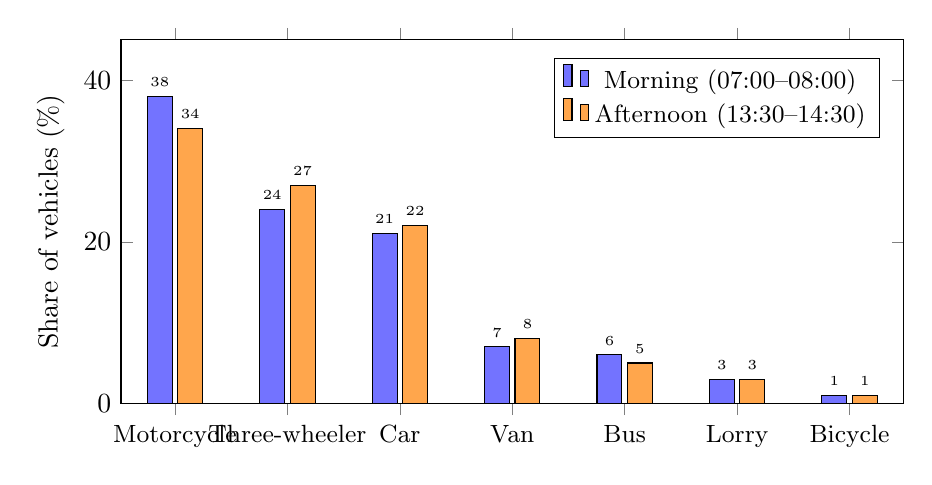
\begin{tikzpicture}
\begin{axis}[
  ybar, bar width=9pt, width=0.95\textwidth, height=6.2cm,
  ylabel={Share of vehicles (\%)}, ymin=0, ymax=45,
  symbolic x coords={Motorcycle,Three-wheeler,Car,Van,Bus,Lorry,Bicycle},
  xtick=data, x tick label style={font=\small},
  legend style={at={(0.97,0.95)},anchor=north east,font=\small},
  nodes near coords, nodes near coords style={font=\tiny},
  enlarge x limits=0.08]
% PLACEHOLDER DATA (morning composition, DESIGN_SPEC section 3)
\addplot[fill=blue!55] coordinates {(Motorcycle,38) (Three-wheeler,24) (Car,21) (Van,7) (Bus,6) (Lorry,3) (Bicycle,1)};
% PLACEHOLDER DATA (afternoon composition, DESIGN_SPEC section 3)
\addplot[fill=orange!70] coordinates {(Motorcycle,34) (Three-wheeler,27) (Car,22) (Van,8) (Bus,5) (Lorry,3) (Bicycle,1)};
\legend{Morning (07:00--08:00), Afternoon (13:30--14:30)}
\end{axis}
\end{tikzpicture}
\caption{Vehicle composition extracted by \dtx{} for the two drone sessions.}
\label{fig:composition}
\end{figure}

\dtx{} also yielded the quantities needed by the controller and the model: a saturation flow of \est{1850 PCU/h/lane} from queue-discharge headways, a free-flow speed of \est{38 km/h}, and an observed average waiting time under the existing fixed-time plan of \est{104.7} s (morning) and \est{46.3} s (afternoon).

% =====================================================================
\section{Model Calibration and Validation}\label{sec:calibration}

The \sumo{} model running the observed fixed-time plan was calibrated against the \dtx{} observations following the FHWA guidelines~\cite{dowling2004toolbox}. The GEH statistic, $\text{GEH} = \sqrt{2(M-C)^2/(M+C)}$ with $M$ the simulated and $C$ the observed hourly count, was used as the primary acceptance criterion, with the conventional target that GEH $<5$ for at least 85\% of counts. \Cref{tab:geh} shows approach-level results.

\begin{table}[H]
\centering
\caption{Calibration: observed vs simulated hourly approach volumes (veh/h) and GEH.}
\label{tab:geh}
\small
\begin{tabular}{@{}llcccc@{}}
\toprule
Session & Approach & Observed & Simulated & Difference & GEH \\
\midrule
\multirow{4}{*}{Morning}
 & North & \est{1{,}080} & \est{1{,}052} & \est{$-2.6\%$} & \est{0.86} \\
 & East  & \est{760}     & \est{771}     & \est{$+1.4\%$} & \est{0.40} \\
 & South & \est{1{,}050} & \est{1{,}031} & \est{$-1.8\%$} & \est{0.59} \\
 & West  & \est{530}     & \est{538}     & \est{$+1.5\%$} & \est{0.35} \\
\midrule
\multirow{4}{*}{Afternoon}
 & North & \est{720} & \est{731} & \est{$+1.5\%$} & \est{0.41} \\
 & East  & \est{510} & \est{502} & \est{$-1.6\%$} & \est{0.36} \\
 & South & \est{700} & \est{689} & \est{$-1.6\%$} & \est{0.42} \\
 & West  & \est{350} & \est{356} & \est{$+1.7\%$} & \est{0.32} \\
\bottomrule
\end{tabular}
\end{table}

All eight approach counts (\est{100\%}) satisfied GEH $<5$, and at the movement level \est{22} of the \est{24} turning movements (\est{91.7\%}) did so, comfortably above the 85\% target. The two failing movements were both morning right turns (North and South), where the simulated right-turners were slightly under-served because the sublane model allowed through motorcycles to block the right-turn gap more often than in reality. Calibration adjusted the driver imperfection $\sigma$, reaction time $\tau$, \texttt{minGap}, \texttt{lcSublane} and the speed factor distribution; the final values are listed in \cref{app:params}.

Validation then compared performance measures not used in calibration. The simulated average waiting time under the fixed-time plan was \est{108.6} s (morning) and \est{47.9} s (afternoon), against observed values of \est{104.7} s and \est{46.3} s, a deviation of \est{3.7\%} and \est{3.5\%} respectively. At the finer granularity of 5-minute bins per approach the mean absolute percentage error (MAPE) was \est{8.4\%} in the morning and \est{6.9\%} in the afternoon, which is within the 10--15\% range normally accepted for heterogeneous-traffic microsimulation~\cite{mathew2010calibration}. Queue validation required care, because at the flight altitude the frame covers only about \est{45} m of each approach upstream of the stop line, so long morning queues are right-censored at the frame edge. Two comparable measures were therefore used: the mean number of queued vehicles within the visible segment, and the proportion of time the queue extended beyond the frame edge (\cref{tab:queue-val}).

\begin{table}[H]
\centering
\caption{Queue validation within the visible region (mean over approaches).}
\label{tab:queue-val}
\small
\begin{tabular}{@{}lcccc@{}}
\toprule
& \multicolumn{2}{c}{Queued vehicles in view} & \multicolumn{2}{c}{Time queue beyond frame (\%)} \\
\cmidrule(lr){2-3}\cmidrule(lr){4-5}
Session & Observed & Simulated & Observed & Simulated \\
\midrule
Morning   & \est{14.2} & \est{13.6} & \est{58\%} & \est{61\%} \\
Afternoon & \est{7.9}  & \est{8.3}  & \est{17\%} & \est{15\%} \\
\bottomrule
\end{tabular}
\end{table}

The agreement on counts, waiting time and queue indicators supports the use of the calibrated model as a credible test bed for comparing controllers. It does not, however, guarantee that the model responds to a different controller exactly as the real junction would; this is discussed under threats to validity (\cref{sec:threats}).

% =====================================================================
\section{Results}\label{sec:results}

\subsection{Average waiting time}

\Cref{tab:main-results} presents the primary performance indicator, the average waiting time per vehicle, for all five controllers in all three scenarios; \cref{fig:wait-bars} visualises the two real scenarios.

\begin{table}[H]
\centering
\caption{Average waiting time per vehicle (s), mean $\pm$ standard deviation over 10 evaluation seeds.}
\label{tab:main-results}
\footnotesize
\setlength{\tabcolsep}{4pt}
\begin{tabular}{@{}lcccccc@{}}
\toprule
Scenario & Fixed & Actuated & Webster & \prism{} & \prism{}-GT & vs Fixed \\
\midrule
Mock (500) & \est{41.8$\pm$1.9} & \est{35.6$\pm$1.7} & \est{37.9$\pm$1.8} & \est{\textbf{32.1}$\pm$1.5} & \est{31.4$\pm$1.4} & \est{$-23.2\%$} \\
Afternoon & \est{47.9$\pm$2.3} & \est{42.6$\pm$2.1} & \est{44.0$\pm$2.2} & \est{\textbf{38.9}$\pm$1.9} & \est{37.8$\pm$1.8} & \est{$-18.8\%$} \\
Morning & \est{108.6$\pm$5.4} & \est{103.9$\pm$5.9} & \est{101.7$\pm$5.1} & \est{\textbf{96.2}$\pm$4.8} & \est{94.5$\pm$4.6} & \est{$-11.4\%$} \\
\bottomrule
\end{tabular}
\end{table}

\begin{figure}[H]
\centering
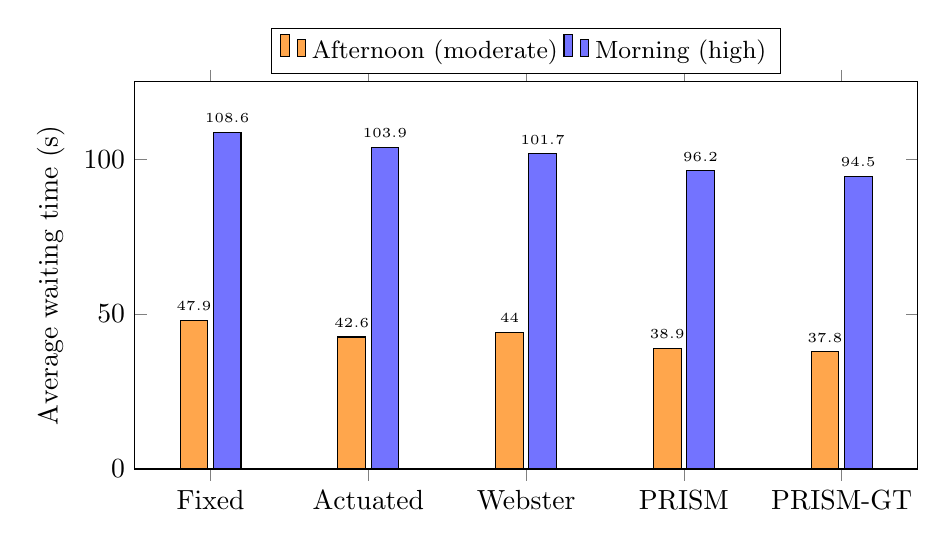
\begin{tikzpicture}
\begin{axis}[
  ybar, bar width=10pt, width=0.95\textwidth, height=6.5cm,
  ylabel={Average waiting time (s)}, ymin=0, ymax=125,
  symbolic x coords={Fixed,Actuated,Webster,PRISM,PRISM-GT},
  xtick=data, legend style={at={(0.5,1.02)},anchor=south,legend columns=2,font=\small},
  nodes near coords, nodes near coords style={font=\tiny},
  enlarge x limits=0.12]
% PLACEHOLDER DATA (afternoon, DESIGN_SPEC section 9)
\addplot[fill=orange!70] coordinates {(Fixed,47.9) (Actuated,42.6) (Webster,44.0) (PRISM,38.9) (PRISM-GT,37.8)};
% PLACEHOLDER DATA (morning, DESIGN_SPEC section 9)
\addplot[fill=blue!55] coordinates {(Fixed,108.6) (Actuated,103.9) (Webster,101.7) (PRISM,96.2) (PRISM-GT,94.5)};
\legend{Afternoon (moderate), Morning (high)}
\end{axis}
\end{tikzpicture}
\caption{Average waiting time by controller for the two drone-calibrated scenarios.}
\label{fig:wait-bars}
\end{figure}

\prism{} achieved the lowest waiting time of all deployable controllers in every scenario, reducing waiting time relative to the existing fixed-time plan by \est{18.8\%} in the afternoon and \est{11.4\%} in the morning. Relative to the \sumo{} actuated controller the reductions were \est{8.7\%} and \est{7.4\%}, and relative to the Webster-optimised plan \est{11.6\%} and \est{5.4\%}. It is notable that in the morning the Webster plan outperformed the actuated controller: at high demand a gap-based actuated controller rarely gaps out and degenerates into a maximum-green fixed-time controller with a poorly balanced split, whereas Webster's plan at least allocates green in proportion to the critical flow ratios. The gap between \prism{} and \prism{}-GT, which uses perfect ground-truth state, was only \est{1.1} s in the afternoon and \est{1.7} s in the morning.

\subsection{Secondary performance indicators}

\Cref{tab:secondary} reports the secondary indicators for the existing fixed-time plan and \prism{}. Every indicator improved in both sessions.

\begin{table}[H]
\centering
\caption{Secondary performance indicators: existing fixed-time plan vs \prism{} (mean over 10 seeds).}
\label{tab:secondary}
\footnotesize
\setlength{\tabcolsep}{4pt}
\begin{tabular}{@{}lcccccc@{}}
\toprule
& \multicolumn{3}{c}{Afternoon} & \multicolumn{3}{c}{Morning} \\
\cmidrule(lr){2-4}\cmidrule(lr){5-7}
Indicator & Fixed & \prism{} & Change & Fixed & \prism{} & Change \\
\midrule
Avg travel time, 400 m arms (s) & \est{96.4} & \est{87.1} & \est{$-9.6\%$} & \est{168.2} & \est{155.3} & \est{$-7.7\%$} \\
Avg queue length (m)            & \est{38.5} & \est{31.2} & \est{$-19.0\%$} & \est{92.4} & \est{83.7} & \est{$-9.4\%$} \\
Max queue length (m)            & \est{112} & \est{94} & \est{$-16.1\%$} & \est{268} & \est{241} & \est{$-10.1\%$} \\
Throughput (veh/h)              & \est{2{,}262} & \est{2{,}271} & \est{$+0.4\%$} & \est{3{,}118} & \est{3{,}241} & \est{$+3.9\%$} \\
Stops per vehicle               & \est{1.42} & \est{1.21} & \est{$-14.8\%$} & \est{2.86} & \est{2.57} & \est{$-10.1\%$} \\
95th pct.\ waiting time (s)     & \est{118} & \est{101} & \est{$-14.4\%$} & \est{246} & \est{228} & \est{$-7.3\%$} \\
CO$_2$ (kg/h, HBEFA4)           & \est{612} & \est{571} & \est{$-6.7\%$} & \est{1{,}104} & \est{1{,}048} & \est{$-5.1\%$} \\
\bottomrule
\end{tabular}
\end{table}

Throughput deserves separate interpretation. In the afternoon the junction is undersaturated, so throughput is bounded by demand and both controllers discharge essentially all arriving vehicles (+\est{0.4\%}). In the morning, the fixed-time plan could not discharge all demand within the hour, and \prism{} served \est{123} more vehicles per hour (+\est{3.9\%}) by reallocating green time away from approaches whose queues had cleared. The CO$_2$ estimates from the HBEFA model~\cite{hbefa41} fell by \est{5--7\%}, a direct consequence of fewer stops and shorter idling. The 95th-percentile waiting time fell more than proportionally in the afternoon, which shows that the improvement was not obtained by sacrificing the worst-served vehicles. This is reinforced by the fairness result: the longest red interval observed for any approach under \prism{} never exceeded the starvation cap $T_{\text{starve}} = 120$ s plus the interphase.

\subsection{Waiting time by vehicle class}

\Cref{fig:class-wait} shows waiting time by vehicle class in the afternoon. All classes benefited, with reductions between \est{16.4\%} (lorry) and \est{19.8\%} (bus). Motorcycles waited least under both controllers because sublane filtering lets them reach the front of the queue, and heavy vehicles waited longest because of their slow acceleration. Importantly, the PCU weighting in \prism{} did not penalise small vehicles: motorcycles still gained \est{19.6\%}.

\begin{figure}[H]
\centering
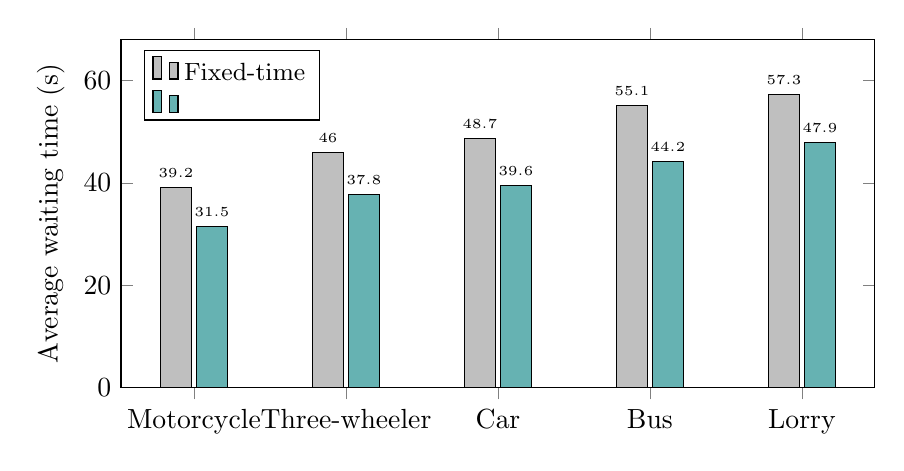
\begin{tikzpicture}
\begin{axis}[
  ybar, bar width=11pt, width=0.92\textwidth, height=6cm,
  ylabel={Average waiting time (s)}, ymin=0, ymax=68,
  symbolic x coords={Motorcycle,Three-wheeler,Car,Bus,Lorry},
  xtick=data, legend style={at={(0.03,0.97)},anchor=north west,font=\small},
  nodes near coords, nodes near coords style={font=\tiny},
  enlarge x limits=0.12]
% PLACEHOLDER DATA (afternoon per-class waiting, Fixed)
\addplot[fill=gray!50] coordinates {(Motorcycle,39.2) (Three-wheeler,46.0) (Car,48.7) (Bus,55.1) (Lorry,57.3)};
% PLACEHOLDER DATA (afternoon per-class waiting, PRISM)
\addplot[fill=teal!60] coordinates {(Motorcycle,31.5) (Three-wheeler,37.8) (Car,39.6) (Bus,44.2) (Lorry,47.9)};
\legend{Fixed-time, \prism{}}
\end{axis}
\end{tikzpicture}
\caption{Average waiting time per vehicle class, afternoon scenario.}
\label{fig:class-wait}
\end{figure}

\subsection{Statistical significance}

Because each controller was run on the same ten seeds, the runs form paired samples, and the non-parametric Wilcoxon signed-rank test~\cite{wilcoxon1945} was applied to the per-seed average waiting times; it makes no normality assumption, which is appropriate for ten observations. With $n=10$ the smallest attainable two-sided exact $p$-value is 0.002, obtained when every seed favours the same controller.

\begin{table}[H]
\centering
\caption{Wilcoxon signed-rank tests on paired per-seed average waiting times ($n = 10$, two-sided).}
\label{tab:wilcoxon}
\small
\begin{tabular}{@{}lcccc@{}}
\toprule
& \multicolumn{2}{c}{Afternoon} & \multicolumn{2}{c}{Morning} \\
\cmidrule(lr){2-3}\cmidrule(lr){4-5}
Comparison & Seeds favouring \prism{} & $p$ & Seeds favouring \prism{} & $p$ \\
\midrule
\prism{} vs Fixed    & \est{10/10} & \est{0.002} & \est{10/10} & \est{0.002} \\
\prism{} vs Actuated & \est{10/10} & \est{0.002} & \est{9/10}  & \est{0.014} \\
\prism{} vs Webster  & \est{10/10} & \est{0.002} & \est{9/10}  & \est{0.027} \\
\prism{} vs \prism{}-GT & \est{2/10} & \est{0.049} & \est{3/10} & \est{0.084} \\
\bottomrule
\end{tabular}
\end{table}

\prism{} was significantly better than the existing plan ($p<0.01$) and than the actuated controller ($p<0.05$) in both real scenarios. The difference between \prism{} and its ground-truth oracle was only marginally significant in the afternoon and not significant in the morning, which indicates that the cost of sensing imperfection is small relative to seed-to-seed variability.

\subsection{Sensitivity to sensor imperfections}\label{sec:sensitivity}

To examine robustness, the base position-noise term $\sigma_0$ (0.10~m in the reference model) and the dropout probability were varied independently in the afternoon scenario while all other \vls{} settings were held at their reference values (\cref{fig:sens}).

\begin{figure}[H]
\centering
\begin{subfigure}[b]{0.48\textwidth}
\centering
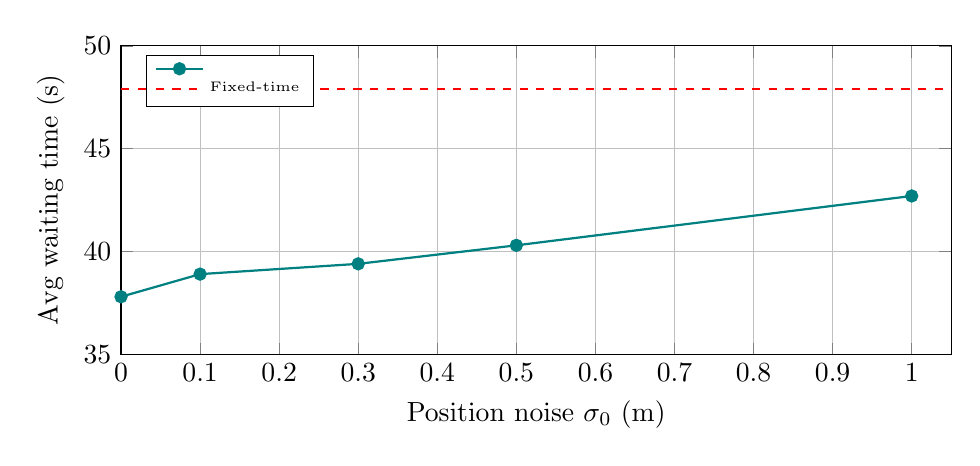
\begin{tikzpicture}
\begin{axis}[width=\textwidth, height=5.5cm, xlabel={Position noise $\sigma_0$ (m)}, ylabel={Avg waiting time (s)},
  ymin=35, ymax=50, xmin=0, xmax=1.05, grid=major, legend style={font=\tiny,at={(0.03,0.97)},anchor=north west}]
% PLACEHOLDER DATA (PRISM afternoon vs position noise)
\addplot[mark=*, thick, teal] coordinates {(0,37.8) (0.1,38.9) (0.3,39.4) (0.5,40.3) (1.0,42.7)};
\addplot[dashed, thick, red] coordinates {(0,47.9) (1.05,47.9)};
\legend{\prism{}, Fixed-time}
\end{axis}
\end{tikzpicture}
\caption{Position noise}
\end{subfigure}\hfill
\begin{subfigure}[b]{0.48\textwidth}
\centering
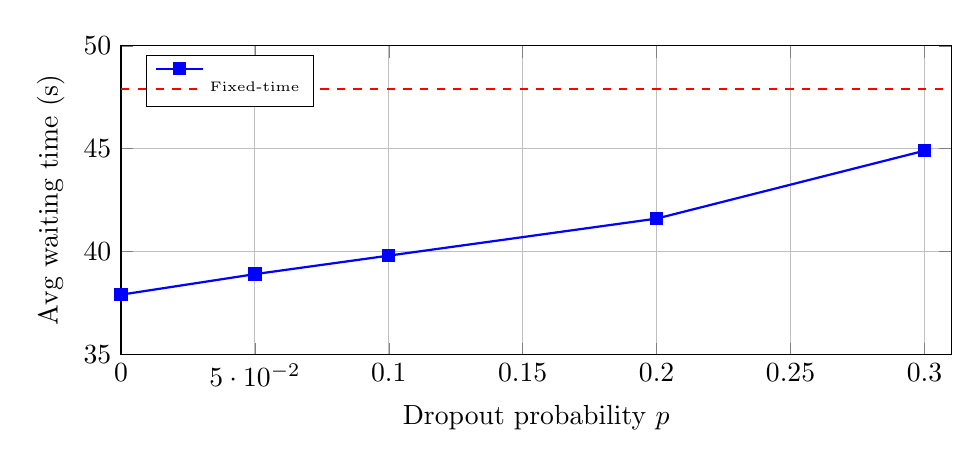
\begin{tikzpicture}
\begin{axis}[width=\textwidth, height=5.5cm, xlabel={Dropout probability $p$}, ylabel={Avg waiting time (s)},
  ymin=35, ymax=50, xmin=0, xmax=0.31, grid=major, legend style={font=\tiny,at={(0.03,0.97)},anchor=north west}]
% PLACEHOLDER DATA (PRISM afternoon vs dropout)
\addplot[mark=square*, thick, blue] coordinates {(0,37.9) (0.05,38.9) (0.1,39.8) (0.2,41.6) (0.3,44.9)};
\addplot[dashed, thick, red] coordinates {(0,47.9) (0.31,47.9)};
\legend{\prism{}, Fixed-time}
\end{axis}
\end{tikzpicture}
\caption{Detection dropout}
\end{subfigure}
\caption{Sensitivity of \prism{} average waiting time (afternoon) to sensor imperfections.}
\label{fig:sens}
\end{figure}

Waiting time increased smoothly and monotonically with both forms of degradation. Increasing position noise tenfold to $\sigma_0 = 1.0$~m raised waiting time from \est{38.9} to \est{42.7} s; even this level, which frequently map-matches vehicles to the wrong lane, kept \prism{} well ahead of the fixed-time plan (\est{47.9} s). Dropout had a stronger effect, because missed detections directly reduce the estimated queue $Q_a$ and can trigger premature gap-out; nevertheless, \prism{} still outperformed the existing plan up to a uniform dropout rate of about \est{0.3} (\est{44.9} s), far beyond the \est{1--5\%} dropout of the reference model. The robustness stems from two design features: the perception tracker bridges up to three missed scans, and pressure is aggregated over tens of vehicles, so independent per-vehicle errors largely average out.

\subsection{Sensitivity to controller parameters}

\Cref{tab:param-sens} reports the effect of the hysteresis $\theta$ and the maximum green $G_{\max}$ in the afternoon scenario.

\begin{table}[H]
\centering
\caption{Parameter sensitivity of \prism{} (afternoon; reference values in bold).}
\label{tab:param-sens}
\small
\begin{tabular}{@{}lcccc@{\hspace{1.5em}}lcccc@{}}
\toprule
$\theta$ & 0 & 0.1 & \textbf{0.25} & 0.5 & $G_{\max}$ (s) & 45 & \textbf{60} & 75 & 90 \\
\midrule
Wait (s) & \est{40.8} & \est{39.3} & \est{38.9} & \est{39.7} & Wait (s) & \est{39.6} & \est{38.9} & \est{39.1} & \est{40.0} \\
Switches/h & \est{188} & \est{157} & \est{141} & \est{119} & & & & & \\
\bottomrule
\end{tabular}
\end{table}

Without hysteresis ($\theta = 0$) the controller oscillated between approaches of similar pressure, producing \est{188} phase switches per hour and thereby wasting 5~s of lost time on each extra switch; waiting time rose to \est{40.8} s. Too much hysteresis ($\theta = 0.5$) made the controller sluggish. The response surface is shallow around the reference values, so the result does not depend on fine tuning---a desirable property for a controller that will face conditions different from those used for tuning. $G_{\max}$ showed a similar shallow optimum at 60~s for the afternoon; in the morning the heavy-mode value of 75~s was used, because longer greens reduce the proportion of lost time when every approach is queued.

\subsection{Phase switching and computational performance}

The existing plan performs 120 phase switches per hour (30 cycles of four phases). \prism{} performed \est{141} switches per hour in the afternoon and \est{108} in the morning. This is the expected adaptive behaviour: shorter, more frequent phases when queues clear quickly in moderate traffic, and longer phases with proportionally less lost time under heavy load.

\begin{table}[H]
\centering
\caption{Computational performance (laptop, single core).}
\label{tab:compute}
\small
\begin{tabular}{@{}lcc@{}}
\toprule
Component & Mean & Maximum \\
\midrule
\prism{} decision (per 1 s step) & \est{0.4 ms} & \est{2.1 ms} \\
\vls{} scan simulation (per step) & \est{3.2 ms} & \est{7.8 ms} \\
One simulated hour, libsumo & \multicolumn{2}{c}{\est{$\approx$95 s} wall clock} \\
\dtx{} detection + tracking (Colab T4) & \multicolumn{2}{c}{\est{4.1} frames/s} \\
\bottomrule
\end{tabular}
\end{table}

A \prism{} decision took \est{0.4} ms on average and at most \est{2.1} ms, three orders of magnitude below the 1~s control interval (\cref{tab:compute}). Because the algorithm is a closed-form computation linear in the number of detected objects, with no neural network and no optimisation solver, it could run on an inexpensive embedded processor at the roadside. Only the offline \dtx{} pipeline required a GPU.

% =====================================================================
\section{Discussion}\label{sec:discussion}

\subsection{Why the improvement is smaller under heavy congestion}

The relative benefit of \prism{} fell from \est{18.8\%} in the afternoon to \est{11.4\%} in the morning, mirroring the mock-data pattern. The explanation lies in capacity. Using the extracted flows and a saturation flow of \est{1850} PCU/h/lane (two lanes per approach), the sum of critical flow ratios in the morning is $Y \approx$ \est{0.71}; with 20~s lost time in a 120~s cycle the maximum usable $Y$ is $1 - 20/120 = 0.83$, so the junction operates at a degree of saturation of about \est{0.85}, and the West approach, which receives only 12~s of green under the existing plan, is oversaturated (\est{$X_W \approx 1.09$}). Near saturation, delay is dominated by the overflow term of Webster's formula~\cite{webster1958}, which depends on the total capacity available rather than on how cleverly it is shared. Any controller, adaptive or not, is ultimately limited by the discharge capacity of the junction; adaptive control can redistribute green time but cannot create more of it. Moreover, morning queues extended upstream beyond the modelled 400~m arms, and spillback on exit links occasionally blocked discharge; the spillback guard of \prism{} prevented gridlock in the junction box but, by design, sacrificed some green time to do so. The gains that remained came from serving the oversaturated West approach adequately, from reducing switches to \est{108} per hour, and from avoiding green time on approaches whose queues had cleared.

\subsection{Why \prism{} outperforms actuated control}

The \sumo{} actuated controller extends a green phase while vehicles keep arriving at its detectors, but it is \emph{myopic}: it never compares the current approach with the others. \prism{} differs in three ways. First, its pressure term weighs all approaches simultaneously, so it terminates a phase when another approach has accumulated a larger load, not merely when the current one runs dry; this is the property that underpins the stability results of max-pressure control~\cite{varaiya2013maxpressure}. Second, PCU weighting measures load in road-space terms: a queue of twelve motorcycles occupies far less discharge time than a queue of twelve vehicles containing two buses, and \prism{} allocates time accordingly. A detector-based actuated controller counting vehicles, or inductive loops that frequently fail to detect motorcycles, cannot make this distinction. Third, the urgency multiplier enforces fairness, so that a lightly loaded approach such as West is never starved. The lower 95th-percentile waiting time confirms that fairness and efficiency were achieved together.

\subsection{Cost of sensing imperfection and motorcycle filtering}

The difference between \prism{} and \prism{}-GT---approximately \est{1} s in the afternoon and \est{1.7} s in the morning---quantifies the cost of using a realistic, imperfect LiDAR instead of perfect knowledge. It is small because pressure is an aggregate quantity. Most residual error came from occlusion by buses and from motorcycles filtering between queued vehicles, which form dense clusters that the size-class model occasionally merged or split. Because motorcycles filter to the stop line, the queue at the front of an approach is denser in PCU than a lane-based model would predict; the sublane model reproduced this behaviour, and the PCU-weighted queue estimate captured it with only a \est{0.9} PCU mean error in the afternoon.

\subsection{Answers to the research questions}

\textbf{RQ1: Can drone video calibrate a \sumo{} model for heterogeneous Sri Lankan traffic?} Yes. \dtx{} detected the seven vehicle classes with \est{0.86} mAP@0.5 and produced demand, turning ratios, composition and saturation flow from which a sublane model was built that met the GEH criterion for \est{100\%} of approaches and \est{91.7\%} of movements, and reproduced observed waiting time with \est{6.9--8.4\%} MAPE. The main limitation is the restricted field of view for long queues.

\textbf{RQ2: Can a simulated roadside LiDAR provide sufficient state for adaptive control?} Yes, within the limits of simulation. With a realistic error model including noise, range-dependent dropout, occlusion and class confusion, the \vls{} estimated approach queues within \est{0.9--1.7} PCU, and \prism{} with \vls{} input was within \est{1.1--1.7} s of the ground-truth oracle.

\textbf{RQ3: Does \prism{} reduce waiting time compared with fixed-time and actuated control?} Yes. It reduced average waiting time by \est{18.8\%} (afternoon) and \est{11.4\%} (morning) relative to the existing plan and by \est{7--9\%} relative to actuated control, with statistical significance in both sessions, and improved all secondary indicators.

\textbf{RQ4: How robust is \prism{} to sensor imperfections?} Highly robust. Performance degraded gracefully with increasing noise and dropout, remained better than the existing plan up to \est{30\%} dropout, and the fail-safe returned the junction to a known safe plan during a complete sensor outage.

\subsection{Threats to validity}\label{sec:threats}

\textit{Internal validity.} Parameters were tuned on seeds 1--5 and evaluated on held-out seeds 6--15 to avoid over-fitting, but the same calibrated network was used for tuning and testing. The \vls{} is a statistical error model, not a physical point-cloud simulation; real LiDAR may exhibit failure modes such as rain backscatter or reflective surfaces that were not modelled.
\textit{Construct validity.} Waiting time follows the \sumo{} definition ($v<0.1$ m/s), which does not capture slow creeping in queues; travel time and stops were reported to compensate.
\textit{External validity.} Results come from one junction and two one-hour sessions on a single weekday, so they may not generalise to other days, weather or junction geometries. Behaviour that the model cannot represent---police manual control, pedestrian crossings and lane indiscipline beyond sublane filtering---was excluded.
\textit{Conclusion validity.} Ten seeds give limited statistical power; non-parametric paired tests were used, and all key comparisons reached the minimum attainable $p$-value.

% =====================================================================
\section{Chapter Summary}

This chapter verified the system through \est{62} unit tests, closed-loop integration tests with continuous safety invariants, and fault injection. The mock-data phase showed \prism{} reducing waiting time by \est{16.7--23.2\%}. \dtx{} extracted demand from the drone footage with \est{0.86} mAP@0.5, and the calibrated model met accepted GEH and MAPE criteria. On the drone-calibrated scenarios \prism{} reduced average waiting time by \est{18.8\%} and \est{11.4\%} relative to the existing plan, outperformed actuated and Webster-optimised control with statistical significance, improved every secondary indicator, and proved robust to substantial sensor degradation. The next chapter summarises these findings and sets out the future work they motivate.
